%!TEX TS-program = pdflatex
% LaTeX-Vorlage zur Erstellung einer Projektarbeit (Dokumentation eines Projekts)
% auf Basis der Vorlage aus dem Kurs ``LaTeX fürs Studium'' für eine
% Abschlussarbeit in der Fakultät Elektrotechnik, Medien und Informatik an der OTH Amberg-Weiden 
% Aktuelle Version: v0.02
% Quelle für natdin.bst: https://www.bibtex.com/s/bibliography-style-din1505-natdin/
%
% Stand: 30.11.2023
%
% Changelog:
%
% v0.01: 03.06.2023, Anpassung der Vorlage für Projektarbeiten (article statt report, keine Titelblätter)
% v0.02; 30.11.2023, Anpassungen für NLP-Projektarbeit
% 
\documentclass[12pt,oneside]{article}
\usepackage[T1]{fontenc}		% Einstellungen fuer Umlaute usw.
\usepackage[utf8]{inputenc}
\usepackage[ngerman]{babel}

\usepackage{parskip}			% Einstellungen fuer Absaetze: Abstand statt Einrueckung

\usepackage[a4paper,			% Papierformat A4
	    left=2.5cm,				% linker Rand
	    right=2.5cm,			% rechter Rand
	    top=1.5cm,				% oberer Rand
	    bottom=1.5cm,			% unter Rand
	    marginparsep=5mm,		% Abstand der Randnotizen
	    marginparwidth=10mm, 	% Breite der Randnotizen
	    headheight=7mm,			% Hoehe der Kopfzeile
	    headsep=1.2cm,			% Abstand der Kopfzeile
	    footskip=1.5cm,			% Abstand der Fusszeile
	    includeheadfoot]{geometry}

\usepackage{fancyhdr}						% Konfiguration von Kopf- und Fusszeilen
\pagestyle{fancy}							% Seitenstil 'fancy'
\fancyhf{}									% vorhandene Einstellungen loeschen
\setlength{\headwidth}{\textwidth}			% Kopf- und Fusszeile so breit wie der Haupttext
\fancyfoot[R]{\thepage} 					% Festlegung des Seitenstils: Seitenzahlen in der Fusszeile rechts
\fancyfoot[L]{\IhreArbeit}					% Kapitelnr. und -Bezeichnung in der Fusszeile links
%\IhreGruppe: 
\fancyhead[L]{\IhrVornameEins\ \IhrNachnameEins}

\renewcommand{\sectionmark}[1]{	    		% Definition der Ausgabe des Kapitels
  \markboth{Abschnitt \thesection. #1}{}}
\renewcommand{\headrulewidth}{0.5pt}		% Trennlinie zwischen Kopfzeile und Haupttext
\renewcommand{\footrulewidth}{0.5pt}		% Trennlinie zwischen Haupttext und Fusszeile
\fancypagestyle{plain}{				     	% Anpassung des Seitenstils 'plain' bei Beginn neuer Kapitel
  \fancyhf{}								% Vorbelegung loeschen
  \fancyfoot[C]{\thepage}					% Seitenzeilen in der Fusszeile mittig
}

%\usepackage{amsmath}			% Pakete fuer den Mathematikmodus
%\usepackage{amssymb}
%\usepackage[intlimits]{empheq}

\usepackage[sc]{mathpazo}		% Schriftart Palatino fuer Haupttext und Mathematikmodus
\usepackage{pifont}				% zusaetzliche Symbole

% \usepackage[format=hang,		% Einstellung fuer Bildunterschriften
            % font={footnotesize},
            % labelfont={bf},
            % margin=1cm,
            % aboveskip=5pt,
            % position=bottom]{caption}

\usepackage{graphicx}							% Einbinden von Graphiken
\usepackage[svgnames,cmyk,table,hyperref]{xcolor} 	% Verwendung von Farben

\definecolor{aoenglish}{rgb}{0.0, 0.5, 0.0}
\definecolor{battleshipgrey}{rgb}{0.52, 0.52, 0.51}
\definecolor{cardinal}{rgb}{0.77, 0.12, 0.23}

%\usepackage{tikz}								% Erstellen von Grafiken
%\usetikzlibrary{positioning,arrows,plotmarks} % TikZ-Bibliotheken
%\usepackage{pgfplots}                           % Darstellung von Plots, Funktionen, Graphen usw.

%
% Weitere Pakete
%
\usepackage{listings}			% Darstellung von Quellcode
\lstloadlanguages{[ISO]C++,Java,XML,[LaTeX]TeX}
\lstset{language=C++,
	numbers = none,
	basicstyle = \small\ttfamily,
	keywordstyle = \color{blue},
	commentstyle = \color{battleshipgrey},
	stringstyle = \color{cardinal},
	columns = flexible,
    captionpos=b,
	showstringspaces = false
}
\lstset{literate=%
	{Ö}{{\"O}}1
	{Ä}{{\"A}}1
	{Ü}{{\"U}}1
	{ß}{{\ss}}1
	{ü}{{\"u}}1
	{ä}{{\"a}}1
	{ö}{{\"o}}1
	{~}{{\textasciitilde}}1
}

\usepackage[square,numbers,sort]{natbib} % Zitationsstil mit Attribut lastchecked
%
%\usepackage[european, siunitx]{circuitikz}	% Darstellung von Schaltungen
%
%\usepackage{enumerate}			% Formatierung nummerierter Listen

% 
% Persoenliche Angaben
% 
\newcommand*{\IhrVornameEins}{Tsvetan}
\newcommand*{\IhrNachnameEins}{Stanchev}
\newcommand*{\IhreGruppe}{Gruppe 1}
\newcommand*{\IhrStudiengang}{Bachelor Künstliche Intelligenz}
\newcommand*{\IhreArbeit}{Projektarbeit Natural Language Processing \& Information Retrieval}
\newcommand*{\IhreSchluesselwoerter}{NLP, LLM, BERT, Evaluation, SQuAD}
\newcommand*{\IhrErstpruefer}{Prof. Dr. Ulrich Schäfer}

\usepackage[bookmarks, raiselinks, pageanchor, % PDF-Einstellungen
            hyperindex, colorlinks,
            citecolor=black, linkcolor=black,
            urlcolor=black, filecolor=black,
            menucolor=black]{hyperref}
\hypersetup{pdftitle={\IhreArbeit},%
          	%pdfauthor={\IhrVorname\ \IhrNachname},
            pdfauthor={\IhrVornameEins\ \IhrNachnameEins{} 
            	\& \IhrVornameZwei\ \IhrNachnameZwei{}
            	\& \IhrVornameDrei\ \IhrNachnameDrei},%
            pdfsubject={\IhreGruppe},%
            pdfkeywords={\IhreSchluesselwoerter}}

%
% Beginn des Textteils
%

\begin{document}
  \thispagestyle{empty}
  \begin{center}
 	\Large
 	Ostbayerische Technische Hochschule Amberg-Weiden\\
 	Fakultät Elektrotechnik, Medien und Informatik\\[.8cm]
 	\large \IhrErstpruefer\\[.8cm]
 	\large Studiengang \IhrStudiengang\\[.8cm] %, \IhreGruppe
 	\Large \IhreArbeit\\[.8cm]
 	%\large \IhrVorname\ \IhrNachname\\[.8cm]
 	\large \IhrVornameEins\ \IhrNachnameEins\\[.8cm]

 	\today\\[2.5cm]
  \end{center}
  
  \tableofcontents

  \clearpage
  
  %
  % Einleitung
  %
  
  \section{Einleitung}
  

Question Answering (QA) ist eine zentrale Aufgabe der natürlichen
Sprachverarbeitung und hat das Ziel, aus einem gegebenen Textkontext
präzise Antworten auf natürlichsprachliche Fragen zu extrahieren oder zu
generieren. Im Gegensatz zu klassischen Information-Retrieval-Systemen,
die lediglich relevante Dokumente zurückliefern, erfordert QA ein
tiefgehendes Sprachverständnis, da die Antwort häufig als spezifischer
Textausschnitt im Kontext identifiziert werden muss. Solche Systeme
finden Anwendung in zahlreichen Bereichen, darunter digitale
Assistenzsysteme, Suchmaschinen, Wissensmanagement und automatisierte
Auskunftssysteme.

Bis vor wenigen Jahren stellte das Fine-Tuning spezialisierter
Transformer-Modelle auf aufgabenspezifischen Datensätzen den
dominierenden Ansatz für Question Answering dar. Modelle wie BERT und
seine Varianten werden dabei gezielt auf annotierten QA-Datensätzen
trainiert, sodass sie lernen, relevante Antwortspannen innerhalb eines
gegebenen Kontextes zu lokalisieren. Diese Methode hat sich insbesondere
für klar definierte Aufgabenstellungen mit strukturierten Eingaben als
sehr leistungsfähig erwiesen.

Mit dem Aufkommen von Large Language Models (LLMs) wie ChatGPT oder
LLaMA-2 hat sich jedoch ein alternativer Ansatz etabliert. Anstatt
Modelle aufgabenspezifisch zu trainieren, können diese großen,
vortrainierten Sprachmodelle mittels sorgfältig formulierter Prompts
dazu angeleitet werden, Fragen direkt auf Basis eines gegebenen
Kontextes zu beantworten. Dieser Prompt-basierte Ansatz verspricht eine
hohe Flexibilität, da kein zusätzliches Training erforderlich ist und
ein einzelnes Modell für eine Vielzahl unterschiedlicher Aufgaben
eingesetzt werden kann.

Ziel dieser Projektarbeit ist es, diese beiden Ansätze systematisch
miteinander zu vergleichen. Dazu werden zwei fine-tuned
Transformer-Modelle, DistilBERT und T5, sowie zwei Large Language
Models, ChatGPT und LLaMA-2-7B-Chat, auf ihre Leistungsfähigkeit im
Question Answering untersucht. Als Evaluationsgrundlage dient der
SQuAD-Datensatz in Version 1.1, der einen etablierten Benchmark für
extraktives Question Answering darstellt. Die Modelle werden anhand
standardisierter Metriken, insbesondere Exact Match und F1-Score,
bewertet, um sowohl die Genauigkeit als auch die inhaltliche
Übereinstimmung der generierten Antworten zu erfassen.

Durch diesen Vergleich soll aufgezeigt werden, inwieweit fine-tuned
Modelle gegenüber prompt-basierten Large Language Models weiterhin
Vorteile bei spezialisierten Question-Answering-Aufgaben besitzen und
welche Stärken und Schwächen sich aus den unterschiedlichen
Modellansätzen ergeben.

  %
  % Projektplanung und Vorgehen
  %
  
  \section{Projektplanung und Vorgehen}

  \textbf{2.1) Zielsetzung des Projekts}

Ziel dieser Projektarbeit ist der Vergleich zweier Ansätze für Question
Answering: speziell auf den SQuAD-Datensatz \citep{rajpurkar2016squad} fine-tuned
Transformer-Modelle (DistilBERT, T5) und große vortrainierte Large
Language Models (ChatGPT, LLaMA-2-7B-Chat), die über geeignete Prompts
gesteuert werden.

Untersucht wird, wie genau diese Modelle identische Kontext-Frage-Paare
beantworten, gemessen anhand der Metriken Exact Match und F1-Score.
Zusätzlich wird ein kleiner Testdatensatz mit 100 Fragen (TD-B)
verwendet, um zu prüfen, ob er vergleichbare Aussagen wie der
vollständige Validierungsdatensatz (TD-A) erlaubt und sich für den
Vergleich mit LLMs eignet.

Damit soll ein fundierter Vergleich zwischen spezialisierten QA-Modellen
und generischen Sprachmodellen ermöglicht werden.

\textbf{2.2) Datensatz}

Als Datengrundlage für diese Projektarbeit wird der Stanford Question
Answering Dataset (SQuAD) Version 1 verwendet. SQuAD besteht aus
Kontextpassagen aus Wikipedia-Artikeln sowie zugehörigen Fragen, deren
Antworten als exakte Textspannen im jeweiligen Kontext annotiert sind.
Der Datensatz ist ein etablierter Standard für die Evaluierung von
Question-Answering-Systemen.

Für die Experimente werden zwei Testdatensätze definiert. Der
vollständige offizielle Validierungsdatensatz von SQuAD wird als TD-A
verwendet und dient zur umfassenden Evaluierung der fine-tuned Modelle
DistilBERT und T5. Zusätzlich wird aus diesem Validierungsdatensatz ein
zufälliger Teiltestdatensatz mit 100 Fragen erzeugt, der als TD-B
bezeichnet wird.

TD-B wird verwendet, um sowohl die fine-tuned Modelle als auch die Large
Language Models ChatGPT und LLaMA-2-7B-Chat unter identischen
Bedingungen zu testen. Da die Auswertung der LLMs manuell
beziehungsweise mit hohem Rechenaufwand erfolgt, ermöglicht TD-B einen
fairen und praktikablen Vergleich aller Modelle. Gleichzeitig erlaubt
der Vergleich der Ergebnisse von TD-A und TD-B eine Bewertung der
Aussagekraft des kleinen Testdatensatzes.

\textbf{2.3) Modelle}

Für den Vergleich werden zwei fine-tuned Transformer-Modelle und zwei
Large Language Models eingesetzt, die unterschiedliche Ansätze für
Question Answering repräsentieren.

DistilBERT \citep{sanh2019distilbert} ist ein kompaktes und effizientes Derivat des BERT-Modells,
das speziell für extraktives Question Answering eingesetzt wird. Das
Modell erhält einen Kontext und eine Frage als Eingabe und bestimmt die
Antwort als zusammenhängende Textspanne innerhalb des Kontexts. Aufgrund
seiner reduzierten Modellgröße eignet sich DistilBERT gut für
effizientes Fine-Tuning und dient in dieser Arbeit als Vertreter
klassischer, aufgabenspezifisch trainierter QA-Modelle.

T5 (Text-to-Text Transfer Transformer) \citep{raffel2020t5} formuliert alle Aufgaben,
einschließlich Question Answering, als Text-zu-Text-Problem. Im
Gegensatz zu DistilBERT erzeugt T5 die Antwort generativ als neuen Text,
anstatt sie direkt aus dem Kontext zu extrahieren. Dadurch kann das
Modell flexibler formulieren, ist jedoch stärker von der Qualität des
Fine-Tunings und der Trainingsdaten abhängig.

Als Vertreter der Large Language Models wird ChatGPT \citep{openai2023chatgpt} verwendet. ChatGPT
ist ein leistungsfähiges, allgemein trainiertes Sprachmodell, das über
ein Prompt dazu angeleitet wird, Fragen auf Basis eines gegebenen
Kontexts zu beantworten. Da es nicht auf den SQuAD-Datensatz fine-tuned
wurde, zeigt es, wie gut ein starkes generisches Sprachmodell ohne
aufgabenspezifisches Training für Question Answering geeignet ist.

Zusätzlich wird LLaMA-2-7B-Chat \citep{touvron2023llama2} eingesetzt, ein frei verfügbares Large
Language Model mit etwa sieben Milliarden Parametern, das für
dialogbasierte Anwendungen optimiert ist. Auch dieses Modell wird
ausschließlich über Prompts gesteuert und nicht weiter fine-tuned. Es
dient als Vergleich zu ChatGPT, um zu untersuchen, wie sich ein offenes,
lokal ausführbares LLM im Vergleich zu einem kommerziellen System
verhält.

Durch diese Modellauswahl wird ein breites Spektrum von spezialisierten
QA-Systemen bis hin zu generischen Sprachmodellen abgedeckt, was einen
aussagekräftigen Vergleich der beiden Ansätze ermöglicht.

\textbf{2.4) Trainingsstrategie für DistilBERT und T5}

Die Modelle DistilBERT und T5 werden mithilfe des
SQuAD-Trainingsdatensatzes fine-tuned, um sie gezielt für die Aufgabe
des Question Answering zu optimieren. Beide Modelle werden aus
vortrainierten Gewichten initialisiert und anschließend auf die
spezifische Struktur von SQuAD angepasst, das aus
Kontext-Frage-Antwort-Tripeln besteht.

Für das Fine-Tuning wird der offizielle Trainingssplit von SQuAD
verwendet, während der Validierungsdatensatz als TD-A zur
Leistungsbewertung während und nach dem Training dient. Die Modelle
werden über mehrere Epochen trainiert, wobei nach jeder Epoche ein
Modell-Checkpoint gespeichert wird. Auf diese Weise kann später der
bestperformende Trainingsstand ausgewählt und für die Evaluation genutzt
werden.

DistilBERT wird als extraktives Modell trainiert, das die Start- und
Endposition der Antwortspanne im Kontext vorhersagt. T5 wird hingegen
als generatives Modell trainiert, das auf Grundlage von Kontext und
Frage eine Textantwort erzeugt. Trotz dieser unterschiedlichen
Ausgabemechanismen werden beide Modelle auf denselben Trainingsdaten
optimiert, wodurch ein fairer Vergleich ermöglicht wird.

Durch diese Trainingsstrategie wird sichergestellt, dass beide
Transformer-Modelle bestmöglich an den SQuAD-Datensatz angepasst sind
und ihre Leistung direkt mit den nicht fine-tuned Large Language Models
verglichen werden kann.

\textbf{2.5) Prompt-Design für LLMs}

Da ChatGPT und LLaMA-2 nicht speziell auf den SQuAD-Datensatz fine-tuned
sind, müssen sie über ein geeignetes Prompt explizit dazu angeleitet
werden, die Aufgabe des Question Answering korrekt auszuführen. Ohne
eine solche Instruktion neigen Large Language Models dazu, erklärende
Texte, Einleitungen oder frei formulierte Antworten zu erzeugen, die
nicht mit dem Antwortformat von SQuAD kompatibel sind.

In dieser Arbeit wird ein festes Prompt-Template verwendet, das jedes
Modell als reinen Antwort-Extraktor definiert. Das Prompt besteht aus
drei zentralen Bestandteilen: dem Kontext, der die relevante Textpassage
enthält, der Frage sowie einer klaren Instruktion, ausschließlich die
exakte Antwortspanne aus dem Kontext zurückzugeben. Zusätzlich wird
festgelegt, dass keine zusätzlichen Wörter ausgegeben werden dürfen und
dass im Fall einer nicht auffindbaren Antwort der Platzhalter
\emph{unknown} zurückzugeben ist.

Dieses strikt formulierte Prompt soll sicherstellen, dass die Ausgaben
der LLMs möglichst gut mit den goldstandardbasierten SQuAD-Antworten
vergleichbar sind und eine automatische Berechnung von Exact-Match- und
F1-Score möglich bleibt.

Für beide Large Language Models, ChatGPT und LLaMA-2-7B-Chat, wird
derselbe Testdatensatz TD-B mit 100 Fragen verwendet. Die generierten
Antworten werden für jedes Modell gespeichert und als JSON-Dateien
abgelegt, sodass sie identisch wie die Ausgaben der fine-tuned Modelle
ausgewertet und verglichen werden können.

\textbf{2.6) Evaluationsstrategie}

Die Leistung aller Modelle wird mithilfe der standardisierten Metriken
Exact Match (EM) und F1-Score bewertet. Der Exact-Match-Wert misst, ob
eine erzeugte Antwort exakt mit der Referenzantwort übereinstimmt,
während der F1-Score auch teilweise korrekte Übereinstimmungen
berücksichtigt. Durch die Kombination beider Metriken lassen sich sowohl
strenge als auch tolerantere Bewertungsaspekte abdecken.

Für alle Modelle wird dasselbe Evaluierungsskript verwendet, um eine
faire und konsistente Auswertung sicherzustellen. Die Ausgaben der Large
Language Models werden vor der Bewertung nachbearbeitet, um zusätzliche
Texte wie Einleitungen oder Erklärungen zu entfernen, sodass nur die
eigentliche Antwortspanne mit den SQuAD-Referenzen verglichen wird.

\textbf{2.7) Vergleichsdesign}

Die beiden fine-tuned Modelle DistilBERT und T5 werden sowohl auf dem
vollständigen Validierungsdatensatz TD-A als auch auf dem
Teiltestdatensatz TD-B evaluiert. Die Large Language Models ChatGPT und
LLaMA-2-7B-Chat werden ausschließlich auf TD-B getestet, da ihre
Auswertung mit höherem manuellem oder rechnerischem Aufwand verbunden
ist.

TD-B dient damit als gemeinsame Vergleichsbasis für alle vier Modelle.
Gleichzeitig erlaubt der Vergleich der Ergebnisse der fine-tuned Modelle
auf TD-A und TD-B eine Bewertung, inwieweit der kleine Datensatz TD-B
repräsentativ für den vollständigen Testdatensatz ist und verlässliche
Rückschlüsse auf die Modellleistung zulässt.
  
  \section{Implementierung}
  
  \textbf{3.1) Datenvorbereitung}

Die Grundlage aller Experimente bildet der SQuAD-v1-Datensatz, der im
JSON-Format vorliegt und für jede Instanz einen Kontext, eine Frage
sowie die zugehörige Referenzantwort enthält. Für die weitere
Verarbeitung werden diese Daten zunächst eingelesen und in eine
einheitliche interne Struktur überführt, bestehend aus Tripeln der Form
(Kontext, Frage, Antwort).

Aus dem offiziellen Validierungsdatensatz wird der vollständige
Testdatensatz TD-A erzeugt. Zusätzlich wird durch zufälliges Ziehen von
100 Einträgen aus TD-A der Teiltestdatensatz TD-B gebildet, der für den
Vergleich mit den Large Language Models verwendet wird. Die zufällige
Auswahl stellt sicher, dass TD-B eine möglichst unverzerrte Stichprobe
des Gesamtdatensatzes darstellt.

Für die fine-tuned Modelle DistilBERT und T5 erfolgt anschließend eine
Tokenisierung der Texte mithilfe der jeweils zugehörigen
HuggingFace-Tokenizer. Dabei werden Kontext und Frage in ein gemeinsames
Eingabeformat überführt, während die Antwort entweder als Textspanne
(DistilBERT) oder als Zieltext (T5) kodiert wird. Durch diese
Vorverarbeitung wird gewährleistet, dass alle Modelle konsistente und
korrekt formatierte Eingaben erhalten und die Daten für Training und
Evaluation vergleichbar bleiben.

\textbf{3.2) Fine-Tuning der Transformer-Modelle DistilBERT und T5}

Für das fine-tuned Question Answering werden die beiden
Transformer-Modelle DistilBERT und T5 verwendet, die unterschiedliche
Ansätze zur Antwortgenerierung verfolgen. DistilBERT wird als
extraktives Modell eingesetzt und sagt die Start- und Endposition der
Antwortspanne innerhalb des Kontexts voraus, während T5 als generatives
Modell eine freie Textantwort aus Kontext und Frage erzeugt.

Beide Modelle werden aus vortrainierten Gewichten initialisiert und
mithilfe des SQuAD-Trainingsdatensatzes weitertrainiert. Die
Tokenisierung und Datenaufbereitung erfolgt modellabhängig, wobei
Kontext und Frage gemeinsam als Eingabe verwendet werden. Das Training
wird über mehrere Epochen durchgeführt, wobei nach jeder Epoche ein
Modell-Checkpoint gespeichert wird. Dadurch können unterschiedliche
Trainingsstände später ausgewählt und reproduzierbar ausgewertet werden.

Die Leistungsüberwachung erfolgt auf dem Validierungsdatensatz TD-A. Der
jeweils bestperformende Checkpoint von DistilBERT und T5 wird
anschließend für die abschließende Evaluation auf TD-A und TD-B
verwendet, um einen fairen Vergleich mit den Large Language Models zu
ermöglichen.

\textbf{3.3) Inferenz mit Large Language Models ChatGPT und LLaMA-2}

Für die Auswertung der Large Language Models werden die zuvor
definierten Prompt-Templates verwendet, die Kontext, Frage und eine
klare Instruktion zur Ausgabe der exakten Antwortspanne enthalten. Diese
Prompts werden automatisch aus dem Testdatensatz TD-B generiert und
bilden die Grundlage für die Inferenz beider LLMs.

Die Auswertung mit ChatGPT erfolgt über das Web-Interface. Die erzeugten
Prompts werden schrittweise in die Benutzeroberfläche eingegeben, und
die resultierenden Antworten werden manuell in strukturierter Form
gespeichert. Dieses Vorgehen entspricht den Vorgaben der
Aufgabenstellung, da für ChatGPT kein programmgesteuerter Zugriff zur
Verfügung steht. Die gesammelten Ausgaben werden anschließend als
JSON-Datei gespeichert, sodass sie automatisiert weiterverarbeitet
werden können.

Für LLaMA-2-7B-Chat wird das Modell lokal auf einem Server mit
GPU-Unterstützung geladen. Die Inferenz auf TD-B erfolgt vollständig
automatisiert, indem alle generierten Prompts sequenziell an das Modell
übergeben werden. Die Antworten werden direkt während der Berechnung in
JSON-Dateien gespeichert. Durch diesen Ansatz ist eine effiziente und
reproduzierbare Auswertung des Modells möglich.

Durch die gemeinsame Verwendung desselben Prompt-Formats und desselben
Testdatensatzes TD-B ist sichergestellt, dass die Ergebnisse von ChatGPT
und LLaMA-2 direkt vergleichbar sind.

\textbf{3.4) Post-Processing}

Die Ausgaben der Large Language Models müssen vor der Evaluation
nachbearbeitet werden, da generische Sprachmodelle häufig zusätzliche
Texte wie Einleitungen, Erklärungen oder Wiederholungen des Prompts
erzeugen. Solche Zusätze sind für die automatische Berechnung der
SQuAD-Metriken ungeeignet, da Exact Match und F1-Score ausschließlich
auf der reinen Antwortspanne basieren.

Bei LLaMA-2 erfolgt diese Nachbearbeitung automatisiert. Nach der
Textgenerierung wird der erzeugte Output so bereinigt, dass nur der
eigentliche Antwortteil erhalten bleibt. Dazu wird beispielsweise alles
vor der letzten Markierung „Answer:`` entfernt, und der Text wird an
Zeilenumbrüchen oder unerwarteten Phrasen abgeschnitten. Auf diese Weise
werden Prompt-Wiederholungen und zusätzliche Erklärungen entfernt, bevor
die Antworten gespeichert und ausgewertet werden.

Bei ChatGPT wird die gewünschte Ausgabeform bereits durch das Prompt
vorgegeben, das explizit die Rückgabe der exakten Antwortspanne ohne
zusätzliche Wörter verlangt. Die Antworten werden anschließend in dieser
Form manuell übernommen und gespeichert. Zusätzlich wird für alle
Modelle, einschließlich DistilBERT und T5, eine Standard-Normalisierung
angewendet, bei der Groß- und Kleinschreibung, Artikel, Satzzeichen und
überflüssige Leerzeichen entfernt werden. Dadurch wird sichergestellt,
dass die berechneten Exact-Match- und F1-Scores die inhaltliche
Übereinstimmung der Antworten korrekt widerspiegeln.

\textbf{3.5) Evaluationsskript}

Die Bewertung aller Modelle erfolgt mithilfe eines einheitlichen
Evaluationsskripts, das die Metriken Exact Match (EM) und F1-Score gemäß
der offiziellen SQuAD-Definition berechnet. Für jede Frage wird die
vorhergesagte Antwort mit einer oder mehreren Referenzantworten
verglichen. Der Exact-Match-Wert ist 1, wenn die normalisierte
Modellantwort exakt mit einer der Referenzantworten übereinstimmt,
andernfalls 0. Der F1-Score wird auf Token-Ebene berechnet und misst die
Überlappung zwischen vorhergesagter und referenzierter Antwort.

Vor der Berechnung werden sowohl Vorhersagen als auch Referenzantworten
normalisiert, indem Groß- und Kleinschreibung vereinheitlicht,
Satzzeichen und Artikel entfernt sowie Leerzeichen standardisiert
werden. Dadurch werden rein formale Unterschiede, die inhaltlich
irrelevant sind, nicht als Fehler gewertet.

Das Evaluationsskript wird für alle Modelle identisch verwendet. Als
Eingaben dienen die SQuAD-konformen JSON-Dateien des jeweiligen
Testdatensatzes (TD-A oder TD-B) sowie die JSON-Dateien mit den
Modellvorhersagen. Für DistilBERT und T5 werden die Vorhersagen direkt
aus den Modellen erzeugt, während für ChatGPT und LLaMA-2 die zuvor
gespeicherten Antwortdateien eingelesen werden. Durch diese einheitliche
Auswertung wird ein fairer und vergleichbarer Vergleich aller vier
Modelle gewährleistet.
  
  \section{Probleme und Diskussion}
  
  \textbf{4.1) Fine-tuned Modelle vs. Large Language Models}

Die Ergebnisse auf dem Teiltestdatensatz TD-B zeigen deutliche
Unterschiede zwischen den spezialisierten, fine-tuned
Question-Answering-Modellen und den allgemeinen Large Language Models.
Wie in den Balkendiagrammen für F1-Score und Exact Match auf TD-B
dargestellt, erzielt DistilBERT die besten Werte unter allen vier
Modellen und übertrifft sowohl ChatGPT als auch LLaMA-2-7B-Chat.
Insbesondere der hohe F1-Score von DistilBERT zeigt, dass das Modell
sehr zuverlässig die relevanten Antwortspannen aus dem Kontext extrahiert.

\begin{figure}[h]
  \centering
  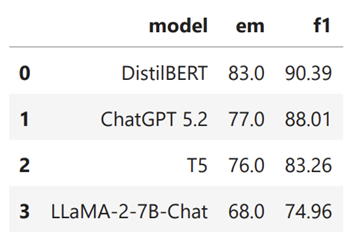
\includegraphics[width=0.4\linewidth]{img_1.png}
  \caption{TD-B: Vergleich der Modelle nach F1-Score und Exact Match.}
  \label{fig:tdb_bar}
\end{figure}

Dieses Ergebnis verdeutlicht den Vorteil spezialisierter,
aufgabenspezifisch trainierter Modelle. DistilBERT wurde direkt auf dem
SQuAD-Datensatz fine-tuned und ist damit optimal auf die Struktur von
Kontext-Frage-Antwort-Tripeln abgestimmt. Im Gegensatz dazu sind ChatGPT
und LLaMA-2 generische Sprachmodelle, die nicht speziell für extraktives
Question Answering trainiert wurden. Trotz ihrer hohen allgemeinen
Sprachkompetenz fehlt ihnen die gezielte Optimierung auf die präzise
Lokalisierung von Antwortspannen, was sich insbesondere im niedrigeren
Exact-Match-Score widerspiegelt.

\begin{figure}[h]
  \centering
  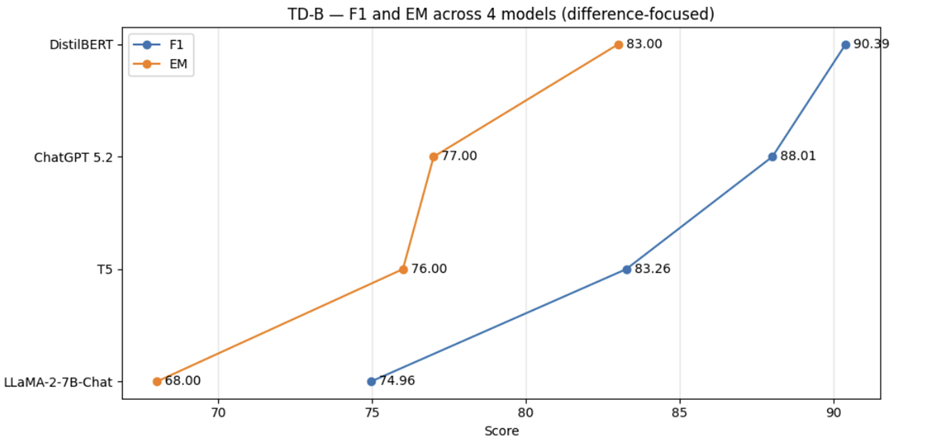
\includegraphics[width=1\linewidth]{img_2.png}
  \caption{TD-B: Vergleich von F1-Score und Exact Match für alle vier Modelle mit Fokus auf die Unterschiede zwischen beiden Metriken.}
  \label{fig:tdb_bar}
\end{figure}

Gleichzeitig zeigt ChatGPT eine bemerkenswert hohe Leistungsfähigkeit,
insbesondere beim F1-Score, der nur geringfügig unter dem von DistilBERT
liegt. Dies deutet darauf hin, dass ChatGPT in der Lage ist, inhaltlich
sehr ähnliche Antworten zu generieren, selbst wenn diese nicht exakt mit
den SQuAD-Referenzantworten übereinstimmen. Die Differenz zwischen F1
und Exact Match bei ChatGPT verdeutlicht dabei den generativen Charakter
des Modells: Häufig werden korrekte Antworten paraphrasiert oder in
leicht abgewandelter Form ausgegeben, was den EM-Wert reduziert, obwohl
die inhaltliche Übereinstimmung hoch bleibt.

Insgesamt zeigen die Ergebnisse, dass fine-tuned QA-Modelle für
strukturierte Benchmarks wie SQuAD weiterhin im Vorteil sind, während
leistungsstarke Large Language Models wie ChatGPT inhaltlich
konkurrenzfähig bleiben, jedoch durch ihre generative Natur bei strengen
Metriken wie Exact Match benachteiligt werden.

\textbf{4.2) Extraktives vs. generatives Question Answering}

Die untersuchten Modelle unterscheiden sich grundlegend in der Art der
Antwortgenerierung. DistilBERT arbeitet als extraktives Modell, das die
Antwort als exakte Textspanne aus dem Kontext auswählt. T5, ChatGPT und
LLaMA-2 sind hingegen generative Modelle, die Antworten in freier
Textform erzeugen und dabei häufig paraphrasieren.

Diese Unterschiede wirken sich deutlich auf die Evaluierungsmetriken
aus. Extraktive Modelle sind strukturell im Vorteil beim
Exact-Match-Score, da ihre Ausgaben direkt mit den Referenzantworten
übereinstimmen können. Generative Modelle erzielen hingegen oft einen
hohen F1-Score, da ihre Antworten inhaltlich korrekt sind, aber in
leicht veränderter Form vorliegen, was den Exact-Match-Wert reduziert.

Dies wird in den Fehleranalysen auf TD-B sichtbar, beispielsweise bei
der Frage zur Apollo-1-Katastrophe, bei der generative Modelle Varianten
wie „O₂`` oder „Oxygen`` ausgeben, während DistilBERT die exakte
Referenz „pure O`` extrahiert. Dadurch zeigt sich, dass generative
Modelle inhaltlich konkurrenzfähig sind, aber durch die strengen
SQuAD-Metriken benachteiligt werden.

\textbf{4.3) TD-A vs. TD-B: Ist der Teiltestdatensatz repräsentativ?}


Ein zentrales Ziel dieser Projektarbeit ist es zu untersuchen, ob der kleine
Teiltestdatensatz TD-B mit nur 100 Fragen aussagekräftige Rückschlüsse
auf das Verhalten der Modelle auf dem vollständigen
Validierungsdatensatz TD-A erlaubt. Diese Frage ist entscheidend, da die Large Language Models ausschließlich auf TD-B evaluiert werden.

\begin{figure}[h]
  \centering
  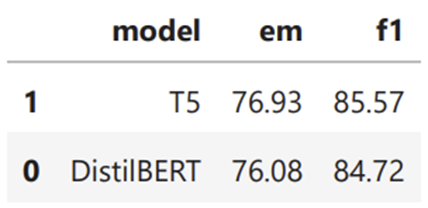
\includegraphics[width=0.3\linewidth]{img_3.png}
  \caption{TD-A: Exact-Match- und F1-Scores der fine-tuned Modelle DistilBERT und T5 auf dem vollständigen Validierungsdatensatz.}
  \label{fig:tdb_bar}
\end{figure}

Der Vergleich der beiden fine-tuned Modelle DistilBERT und T5 auf TD-A
und TD-B zeigt jedoch, dass TD-B nicht vollständig repräsentativ ist.
Auf dem vollständigen Datensatz TD-A erzielt T5 einen leicht höheren
F1-Score als DistilBERT (85.57 vs. 84.72), was darauf hindeutet, dass T5 insgesamt etwas besser generalisiert. Auf TD-B kehrt sich dieses
Verhältnis jedoch um: DistilBERT erreicht hier deutlich höhere Werte als T5 (90.39 vs. 83.26 F1), ebenso beim Exact-Match-Score.

\begin{figure}[h]
  \centering
  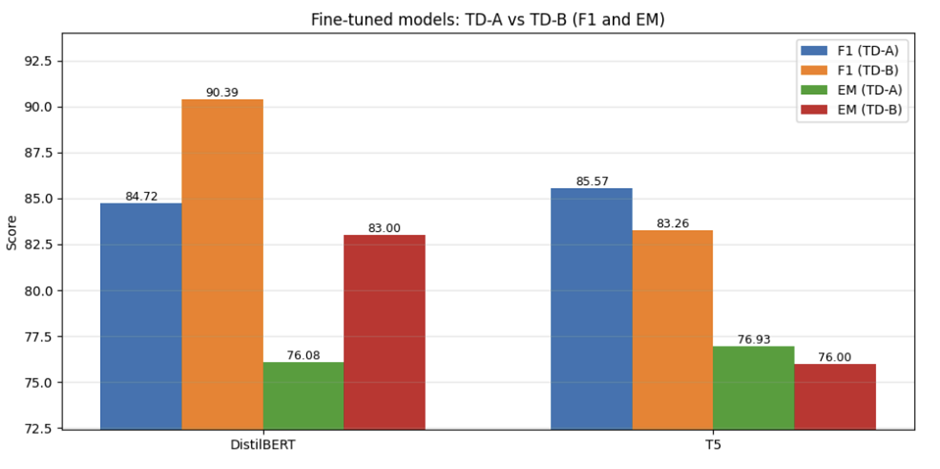
\includegraphics[width=0.8\linewidth]{img_4.png}
  \caption{Vergleich der fine-tuned Modelle DistilBERT und T5 auf TD-A und TD-B (Exact Match und F1-Score).}
  \label{fig:tdb_bar}
\end{figure}

Diese Rangänderung ist in der Abbildung \emph{„Fine-tuned models: TD-A
vs. TD-B (F1 and EM)''} klar sichtbar und zeigt, dass der kleine
Testdatensatz eine verzerrte Stichprobe darstellt. Offenbar enthält TD-B
überdurchschnittlich viele Fragen, die gut zu den Stärken von DistilBERT
passen, während T5 dort schlechter abschneidet als auf dem vollständigen
Datensatz.

Damit lässt sich festhalten, dass TD-B zwar für einen praktischen
Vergleich mit den Large Language Models notwendig ist, jedoch nur
eingeschränkt als repräsentative Näherung für TD-A betrachtet werden
kann. Die Ergebnisse auf TD-B müssen daher mit Vorsicht interpretiert
werden, insbesondere wenn Modelle auf TD-A und TD-B unterschiedlich
gerankt werden.

\textbf{4.4) Übereinstimmung zwischen den Modellen}

Neben den absoluten Leistungswerten ist auch interessant, wie ähnlich
sich die Modelle in ihrem Antwortverhalten sind. Dazu wird auf TD-B eine
paarweise Übereinstimmungsanalyse durchgeführt, bei der gemessen wird,
wie oft zwei Modelle für dieselbe Frage nach Normalisierung exakt
dieselbe Antwort liefern.

Die resultierende Übereinstimmungsmatrix zeigt, dass DistilBERT und T5
die höchste gegenseitige Übereinstimmung aufweisen. Dies ist zu
erwarten, da beide Modelle auf demselben SQuAD-Datensatz fine-tuned
wurden und daher ähnliche Antwortstrategien gelernt haben. Ihre
Antworten stimmen deutlich häufiger überein als die Antworten der Large
Language Models mit denen der fine-tuned Modelle.

Im Gegensatz dazu zeigen ChatGPT und LLaMA-2 eine geringere
Übereinstimmung mit DistilBERT und T5. Dies deutet darauf hin, dass die
LLMs die Fragen anders interpretieren oder alternative Formulierungen
und Antwortspannen wählen. Besonders LLaMA-2 weicht häufig von den
extraktiven Modellen ab, was mit seiner generativen und weniger stark
auf SQuAD abgestimmten Natur erklärt werden kann.

\begin{figure}[h]
  \centering
  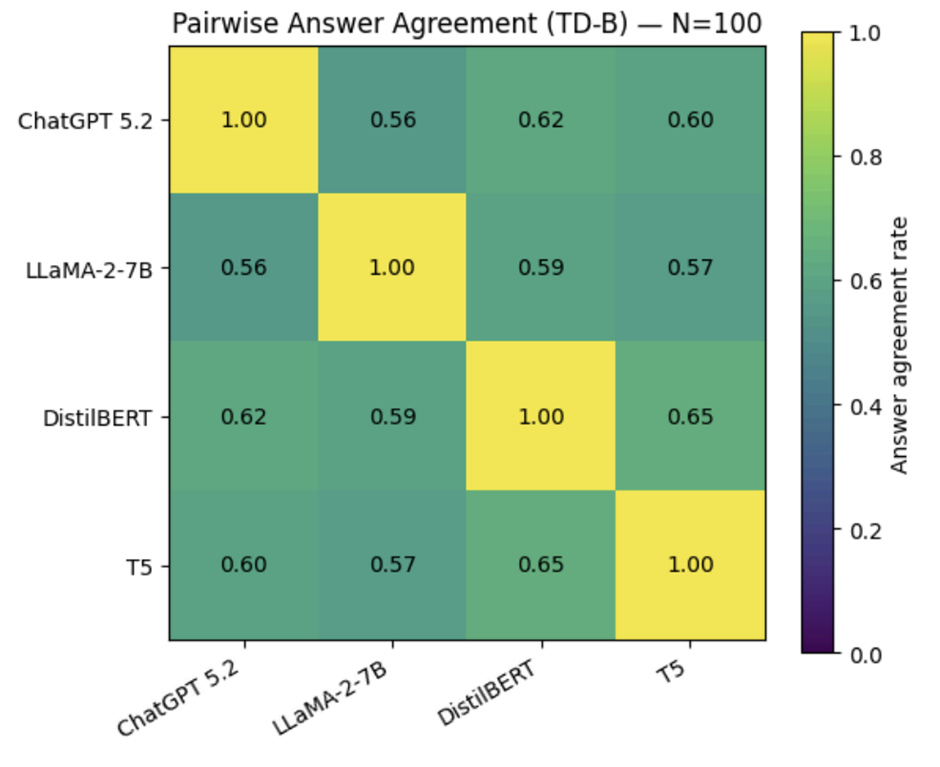
\includegraphics[width=0.5\linewidth]{img_5.png}
  \caption{Paarweise Übereinstimmung der Modellantworten.}
  \label{fig:tdb_bar}
\end{figure}

Diese Analyse bestätigt, dass fine-tuned QA-Modelle ein konsistenteres
und stärker standardisiertes Antwortverhalten zeigen, während Large
Language Models größere Variabilität aufweisen. Dies trägt zusätzlich
dazu bei, die Unterschiede zwischen spezialisierten und generischen
Modellen über reine F1- und EM-Werte hinaus sichtbar zu machen.

\textbf{4.5) Antwortstil und Ausgabelänge}

Die Modelle unterscheiden sich nicht nur in ihrer Genauigkeit, sondern
auch in ihrem Antwortstil. Die Analyse der Antwortlängen auf TD-B zeigt,
dass ChatGPT und LLaMA-2 im Durchschnitt längere und variablere
Antworten erzeugen als die fine-tuned Modelle DistilBERT und T5. Dies
ist eine Folge ihres generativen Charakters, bei dem Antworten häufig
neu formuliert oder erweitert werden.

\begin{figure}[h]
  \centering
  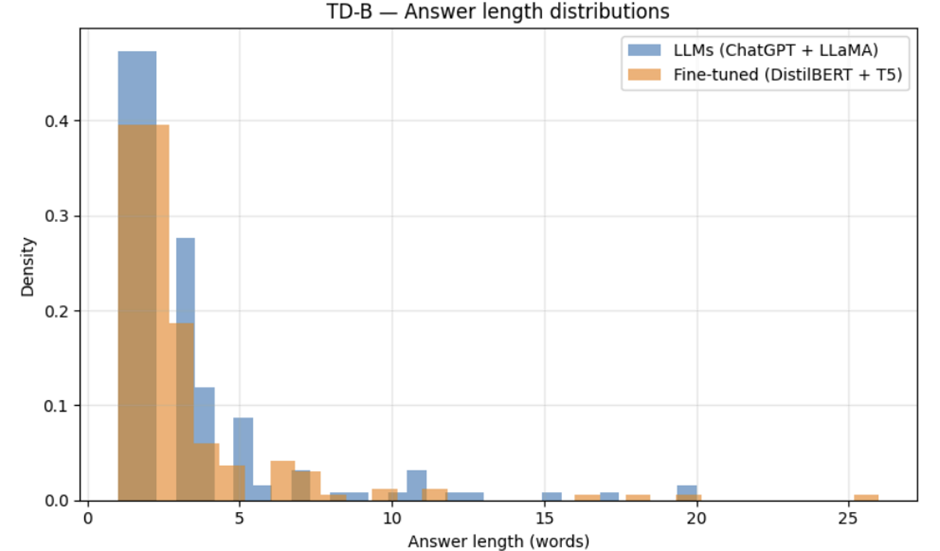
\includegraphics[width=1\linewidth]{img_6.png}
  \caption{Verteilung der Antwortlängen auf TD-B für Large Language Models und fine-tuned Modelle.}
  \label{fig:tdb_bar}
\end{figure}

Im Gegensatz dazu liefern die fine-tuned Modelle meist kurze und präzise
Textspannen, die näher an den annotierten SQuAD-Antworten liegen.
Dadurch sind sie insbesondere bei strengen Metriken wie Exact Match im
Vorteil. Die Verteilung der Antwortlängen bestätigt somit die
unterschiedlichen Eigenschaften von generativen und extraktiven Modellen
im Question Answering.

\textbf{4.6) Typische Fehlerfälle und schwierige Fragen}

Die Analyse der schwierigsten Fragen in TD-B zeigt, dass bestimmte
Fragestellungen selbst für leistungsstarke Modelle problematisch sind.
Besonders auffällig ist, dass bei einigen Fragen alle vier Modelle
versagen oder nur sehr geringe F1-Werte erzielen. Diese Fälle treten
häufig auf, wenn die Antwort stark von der exakten Formulierung der
Referenz abhängt oder mehrere semantisch ähnliche Varianten existieren.

Ein typisches Beispiel ist die Frage nach dem chemischen Element der
Apollo-1-Katastrophe. Während DistilBERT die Referenz „pure O`` korrekt
extrahiert, geben die generativen Modelle Varianten wie „O₂`` oder
„Oxygen`` aus. Obwohl diese Antworten inhaltlich korrekt sind, werden
sie aufgrund der strengen SQuAD-Metriken als falsch oder nur teilweise
korrekt bewertet. Ähnliche Effekte treten bei anderen Fragen auf, bei
denen generative Modelle paraphrasieren oder zusätzliche Informationen
einfügen.

Darüber hinaus zeigen einige Fragen, dass alle Modelle Schwierigkeiten
haben, wenn die relevante Information im Kontext nur indirekt oder über
mehrere Sätze verteilt enthalten ist. In solchen Fällen kommt es sowohl
bei extraktiven als auch bei generativen Modellen zu Fehlzuordnungen
oder unvollständigen Antworten. Diese Fehleranalyse verdeutlicht, dass
die Grenzen der Modelle nicht nur durch ihre Architektur, sondern auch
durch die Struktur und Eindeutigkeit der zugrunde liegenden Texte
bestimmt werden.

\textbf{4.7) Einschränkungen der Studie}

Trotz der systematischen Auswertung unterliegen die Ergebnisse dieser
Projektarbeit mehreren Einschränkungen. Eine zentrale Limitation ist die
geringe Größe des Teiltestdatensatzes TD-B, der nur 100 Fragen umfasst.
Wie in der Analyse gezeigt wurde, ist TD-B nicht vollständig
repräsentativ für den vollständigen Validierungsdatensatz TD-A, was die
Aussagekraft des Vergleichs mit den Large Language Models einschränkt.

Eine weitere Einschränkung betrifft die Nutzung von ChatGPT, dessen
Auswertung aufgrund fehlender Programmierschnittstellen manuell über das
Web-Interface erfolgen musste. Obwohl ein festes Prompt-Template
verwendet wurde, kann dieser manuelle Prozess zu leichten Variationen
oder Übertragungsfehlern führen.

Zudem reagieren Large Language Models empfindlich auf die genaue
Formulierung des Prompts. Andere Prompt-Varianten hätten möglicherweise
zu abweichenden Ergebnissen geführt, was die Vergleichbarkeit weiter
beeinflussen kann. Schließlich wurden ChatGPT und LLaMA-2 nicht auf
SQuAD fine-tuned, sondern ausschließlich im Zero-Shot-Prompting
eingesetzt, was ihre Leistung im Vergleich zu den speziell trainierten
Modellen grundsätzlich limitiert.

Diese Einschränkungen sollten bei der Interpretation der Ergebnisse
berücksichtigt werden und zeigen zugleich Ansatzpunkte für zukünftige,
umfassendere Untersuchungen auf.
  
  \section{Zusammenfassung und Ausblick}

  In dieser Projektarbeit wurde ein Vergleich zwischen fine-tuned
Transformer-Modellen und Large Language Models für die Aufgabe des
Question Answering auf dem SQuAD-Datensatz durchgeführt. Die beiden
spezialisierten Modelle DistilBERT und T5 wurden auf SQuAD fine-tuned
und auf dem vollständigen Validierungsdatensatz TD-A sowie auf einem
kleineren Teiltestdatensatz TD-B evaluiert. ChatGPT und LLaMA-2-7B-Chat
wurden mithilfe eines festen Prompt-Templates ausschließlich auf TD-B
getestet.

Die Ergebnisse zeigen, dass das fine-tuned Modell DistilBERT auf TD-B
die beste Leistung erzielt und beide Large Language Models übertrifft.
ChatGPT erreicht jedoch einen vergleichbaren F1-Score, was auf eine hohe
inhaltliche Qualität seiner generierten Antworten hinweist, auch wenn
diese aufgrund von Paraphrasierungen häufiger beim Exact-Match-Score
benachteiligt werden. Der Vergleich von TD-A und TD-B hat zudem gezeigt,
dass der kleine Teiltestdatensatz nicht vollständig repräsentativ ist,
da sich die Rangfolge der fine-tuned Modelle zwischen beiden Datensätzen
ändert.

Für zukünftige Arbeiten wäre es sinnvoll, größere und mehrere zufällige
Teiltestdatensätze zu verwenden, um robustere Aussagen über die
Leistungsfähigkeit der Modelle zu ermöglichen. Zudem könnte eine
systematische Untersuchung unterschiedlicher Prompt-Varianten für Large
Language Models durchgeführt werden. Schließlich wäre auch ein
Fine-Tuning von LLMs auf SQuAD oder ähnlichen Datensätzen ein
interessanter Ansatz, um den Leistungsunterschied zwischen
spezialisierten und generischen Modellen weiter zu untersuchen.
  
   
  %
  % Literatur 
  %

  \phantomsection
  \addcontentsline{toc}{section}{Literatur}
  \bibliographystyle{natdin}
  \bibliography{quellen}
  

%\input{anhang} % zum Beispiel hier ChatGPT-Chatprotokolle einbinden (als extra-Datei)

\end{document}
